\pagestyle{empty}
\cleardoublepage
\pagestyle{fancy}

\chapter{METODOLOGIA}\label{cap3}

\section*{WEB SCRAPING}

O surgimento da internet, em particular a Web (\emph{Web Wide Word}) trouxe um crescimento exponencial nas disposições de informações. Embora muitas dessas informações sejam úteis, elas raramente estão de uma forma que podemos utilizá-las, pois ainda é comum pessoas gastarem horas na coleta manual de dados de páginas da web. Especificamente, apesar de disponibilidade, poucos trabalhos acadêmicos em Economia utilizam desta fonte de dados para análise econômica empírica. Tal característica pode ser dada pela dificuldade dos pesquisadores na área em lidar com linguagem de programação que demandam maior conhecimento de computação. 

Em recente publicação, \citet{varian2014big} salienta que as técnicas utilizadas na Ciência da Computação e outras áreas correlatas para manipular e analisar dados, têm muito a oferecer. \citet{varian2014big} defende que economistas deveriam conhecer melhor esses métodos e usá-los em seus trabalhos. Além disso, \citet{varian2014big} cita a comumente colaboração entre os departamentos de Ciência da Computação e Estatística nas universidades dos EUA. Porém, o autor espera que em um futuro próximo os estudantes de econometria tenham maior colaboração com esses perfis e assim, contribuir para a pesquisa econômica empírica.

Uma metodologia que facilita o processo de coleta de dados da web é conhecida como \emph{web scraping} que envolve escrever algoritmos que executam automaticamente o que nós fazemos manualmente quando navegamos por uma página de um site de e-commerce, por exemplo. Além disso, necessita-se de pouco conhecimento em programação para iniciar o processo de coleta de dados da internet. Segundo \citet{manning2008introduction} \emph{web scraping} é o processo de tirar informações desestruturadas de páginas da web e transformá-las em informações estruturadas que podem ser usadas para análise. 

A maior parte das páginas de sites são construídas usando uma linguagem de codificação estruturada chamada de \emph{HyperText Markup Language} (HTML). Este código tem “\emph{tags}”, tais como $<center>$ e $<bold>$, que determinam o estilo e localização do texto em uma página. Estas \emph{tags} tendem a permanecer constantes ao longo do tempo, uma vez que proporcionam um “\emph{look and feel}” distinto para cada página. Por contraste, a informação dentro dessas \emph{tags}, tais como preço de produtos, mudam ao longo do tempo. O software de \emph{scraping} pode ser ensinado a utilizar as \emph{tags} em HTML pata localizar informações relevantes sobre um produto e guarda-las em um banco de dados. A repetição desse processo todos os dias produz um banco de dados em formato de painel com um registro por produto por dia. Em adição, o endereço da página (URL) onde cada produto é localizado pode ser usado para classificar produtos em categorias padronizadas. 

\begin{figure}[htbp]
  \centering
  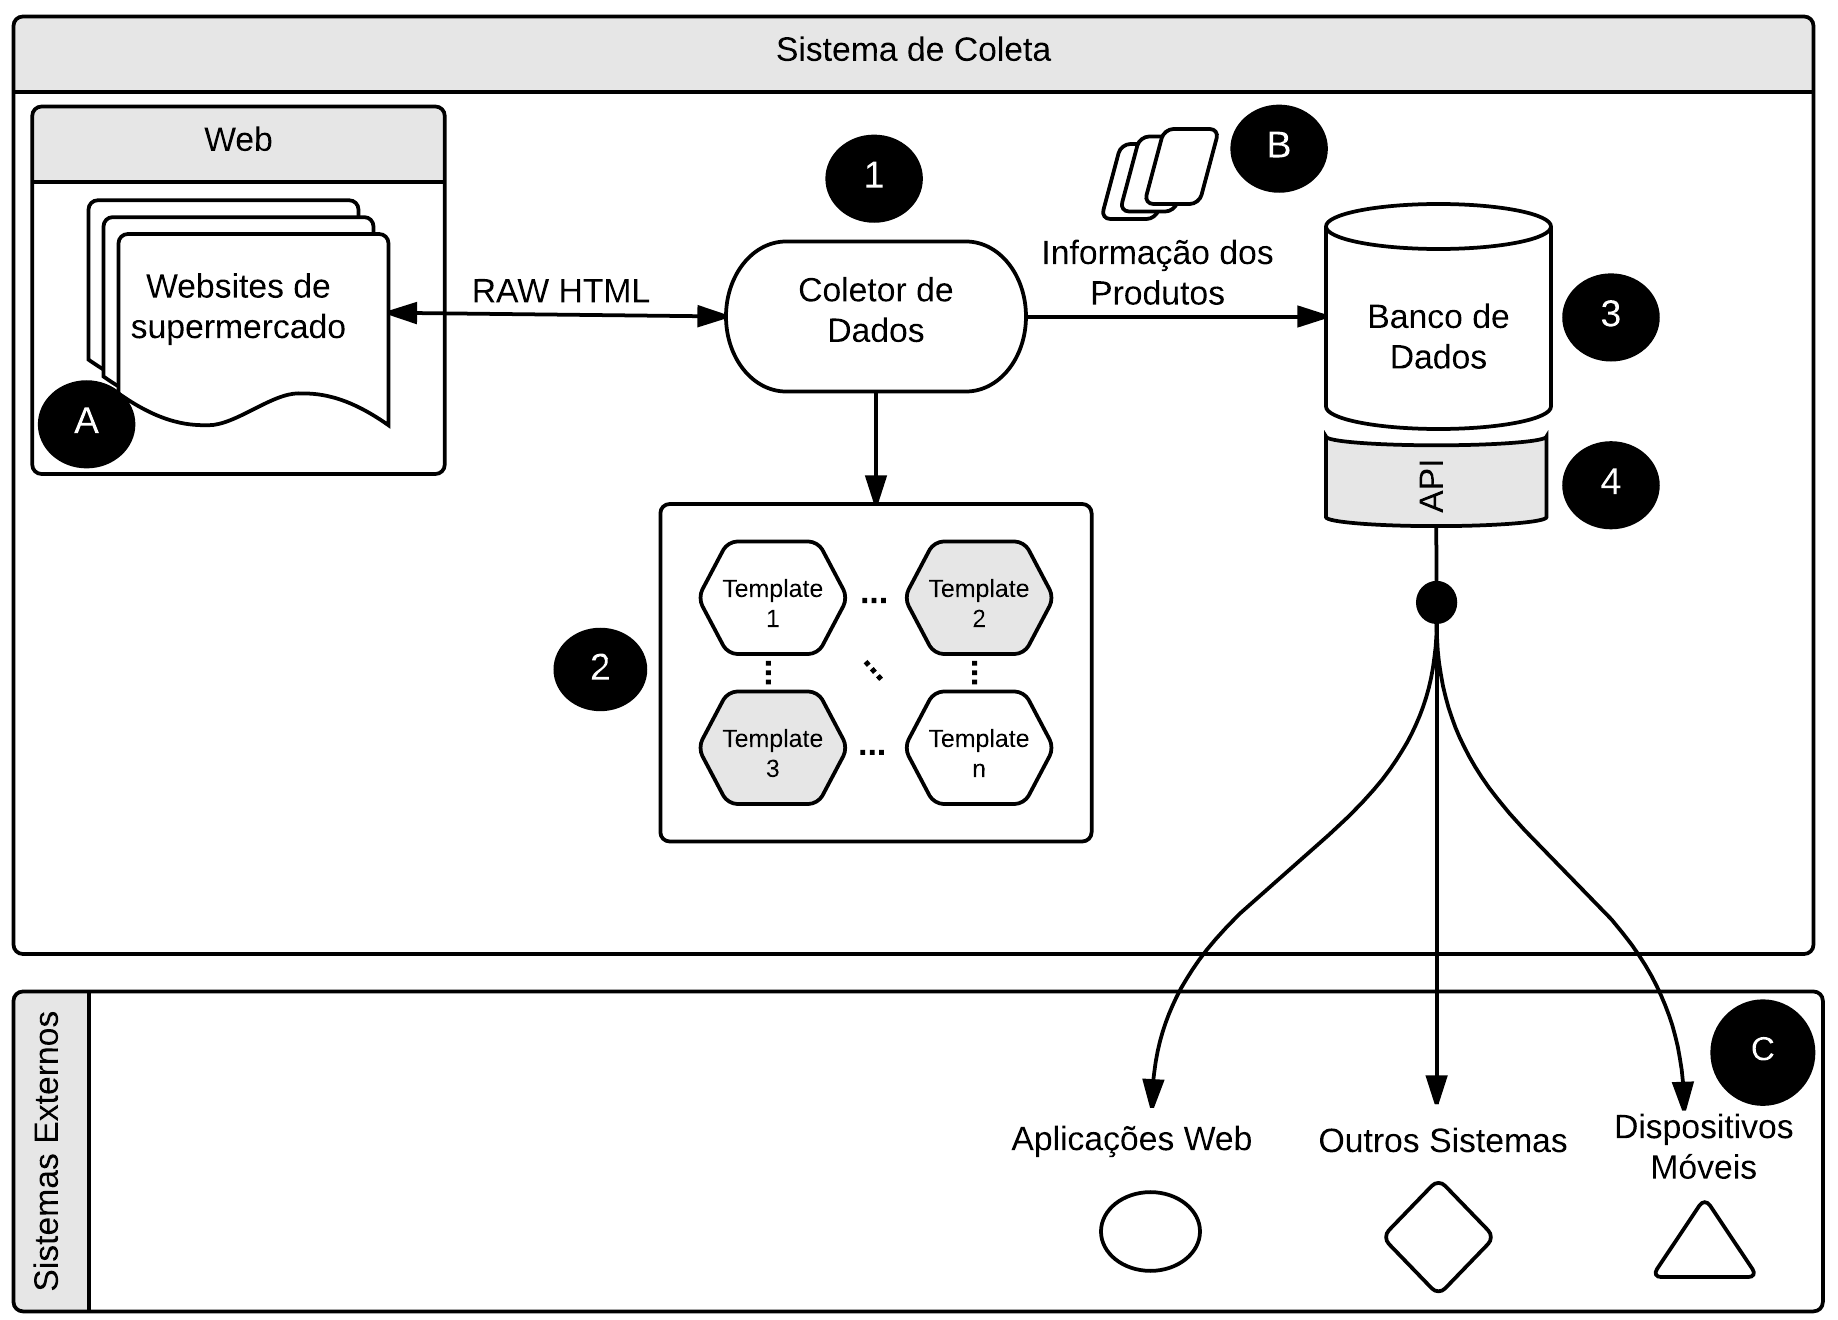
\includegraphics[width=\textwidth]{WebScraping}
  \caption[Figura Simples]{Arquitetura do Sistema de Coleta e Disponibilização dos Dados}
  \label{fig:01}
\end{figure}

Através de um coletor é possível arquiteturar e executar de forma lógica e escalável todo esse processo. Para que um coletor seja funcional é necessário que o mesmo seja capaz de interagir com páginas da Web, extrair a informação de interesse e estruturar e armazenar os dados para futuras consultas. Em geral, exemplos corriqueiros de coletores podem ser citados como os desenvolvidos pelo Google e Microsoft para atuar na procura por páginas da internet ou outros mais específicos para coleta de preços de produtos como os portais de agregadores como Bom de Faro, Buscapé dentre outros. Assim, como \citet{cavallo2010scraped}, o presente projeto de tese busca de forma inovadora para a economia brasileira, explorar preços coletados de sites de supermercados, farmácias, companhia de energia elétrica, lojas de varelo online, lojas de roupas e calçados, entre outros, e propõe o uso de um sistema de coleta como o apresentado a seguir. 

O sistema de coleta de preços está apresentado na Figura~\ref{fig:01}. O coletor recebe como entrada os templates dos sites que se deseja coletar e produz como resposta informações estruturadas com os atributos dos produtos. Para que o coletor seja capaz de realizar a tarefa de extração de informação, o mesmo deve apresentar os seguintes componentes: um componente centralizado capaz de ler instruções e aplicar regras para extração (1 - módulo coletor de dados); ter um conjunto de regras que descreva de forma não ambígua como realizar a coleta dos dados e os atributos de interesse (2 - templates dos webistes de supermercado, por exemplo); ter um banco de dados capaz de lidar com as características dos dados armazenados (3 - módulo de banco de dados); ter uma interface para facilitar o acesso aos dados por meio de outras aplicações ou sistemas web (4 - módulo de disponibilização da informação). Dessa forma, o coletor (1) é o centralizador do processo de coleta de dados, fazendo a interação com os templates (2), os webistes (A) e o módulo de banco de dados (3). Em resumo, o coletor através de um algoritmo inicia o processo de coleta carregando em uma lista os templates de coleta dos websites (2) e em seguida através de um processo iterativo visita o website, coleta os documentos de interesse e realiza a extração das informações indicadas pelo template. Ao final da coleta os dados são estruturados em um formato de documento denominado JSON e armazena-os em um banco de dados NoSQL adequado a essa estrutura de dados. O processo se repete para cada template até que todos os templates sejam avaliados. O algoritmo que descreve esse processo é apresentando em Algoritmo 1. Por fim, além da coleta em si, há um módulo para disponibilizar o acesso a informação coletada. Esse módulo (4) é responsável por permitir de forma segura e racional o uso dos dados coletados por diferentes sistemas e aplicações web existentes (C).

Segundo \citet{cavallo2010scraped}, preços coletados da internet possuem duas desvantagens: Primeiro, percentual menor de empresas disponibiliza seus produtos e preços na internet em comparação com as lojas físicas. Tal limitação pode ser minimizada ao longo do tempo com uma maior oferta de produtos e serviços na internet. Segundo, os preços coletados da internet não incluem informações sobre as quantidades vendidas o que impede de obter market share e estimativas de elasticidade.

Avaliações futuras precisarão ser feitas de forma que seja capaz explorar se os preços online e off-line se comportam similarmente. Preocupado com tal validação, \citet{cavallo2010scraped} fez pesquisa de preços nas lojas físicas dos supermercados utilizados para coleta de dados da internet. Desta forma, o autor examinou se os preços dos produtos nas lojas físicas eram similares aos preços nos sites. Uma importante característica é que um alto percentual de produtos vendidos nas lojas físicas também era comercializado nos sites em todos os países. O autor comparou os preços tanto em termo de nível quanto em tamanho e intervalo de tempo de alterações nos preços. Tal comportamento é muito importante para a avaliação de rigidez nos preços. Para tanto, o autor criou uma série de mudança de preços para cada produto que recebe valor 1 se o preço aumentou, 0 se o preço permaneceu constante e -1, caso contrário.  Assim, foi possível avaliar se os preços dos produtos nas lojas físicas são semelhantes em nível e em direção de mudança para cada produto e supermercado dos países avaliados por \citet{cavallo2010scraped}.

Não obstante, \citet{cavallo2010scraped} apresenta algumas vantagens dos preços coletados da internet que os fazem uma fonte única de informação para análise de rigidez nos preços. Primeiro, pode-se obter preços diários para os produtos e serviços e por conseguinte, reduzir medidas de erro em relação à frequência de cálculo da inflação, analisar promoções de produtos, controles e sincronização nos preços. Segundo, os dados estão disponíveis para vários países, com maior facilidade de acesso e possibilidade de comparação entre países. Terceiro, existem informações detalhadas sobre cada produto e não há substituições forçada de itens como ocorre em estatísticas oficiais de inflação. Por fim, preços coletados da internet estão viáveis em tempo real, sem qualquer atraso para acessá-los. Isto pode ser usado para providenciar estimativas de rigidez nos preços em tempo real.
  
\section*{ÍNDICE DE PREÇOS ONLINE}
  
Para calcular o índice de preços online que será comparado com o Índice Nacional de Preços ao Consumidor Amplo (IPCA) e Índice Nacional de Preços ao Consumidor (INPC) divulgados pelo Instituto Brasileiro de Geografia e Estatística (IBGE), utilizaremos a abordagem proposta por \citet{cavallo2010scraped}.
  
Assim, o índice de preços usa a combinação de dados online e as estruturas de ponderação oficiais do IBGE para as categorias da “cesta de mercadorias”\footnote[1]{Segundo o \citet{ibgemetodos} os índices constituem uma medida síntese de movimento de preços de um conjunto de bens e serviços, chamado “cesta de mercadorias”, representativo de um determinado grupo populacional, em certo período de tempo} de cada índice de inflação. Maiores detalhes sobre a metodologia de coleta e cálculo do IPCA e INPC podem ser obtidas no~\ref{ap1}. Dados diários serão utilizados para construir o índice de preços online o que é útil para observar padrões de curto prazo nos dados que ajudam a validar as informações online. 
  
O índice de preço online será calculado utilizando os preços de todos os produtos disponíveis para compra em cada site. Isto implica que a cesta de bens muda dinamicamente ao longo do tempo podendo um produto aparecer ou desaparecer da cesta a qualquer momento devido à disponibilidade ou indisponibilidade no site. Além disso, o número de preços por produto tende a ser muito maior o que os coletados usualmente pelos órgãos governamentais. 
Para construir o índice, mudanças de preço são calculadas em nível de produto, então as médias dentro das categorias usando média geométrica ponderada e finalmente agregado entre categorias com uma média aritmética ponderada. Em particular, o primeiro passo é obter a média geométrica ponderada das mudanças nos preços na categoria $j$ para cada dia $t$:

\begin{equation}\label{eq1}
R_{t,t-1}^{j}=\prod_{i}\left(\frac{p_{t}^{t}}{p_{t-1}^{i}}\right)^{\nicefrac{1}{n_{j,t}}}
\end{equation}

\noindent onde $p_{t}^{i}$ é o preço do bem $i$ no tempo $t$, $n_{j,t}$ é o número de produtos na categoria $j$ que estão presentes na amostra neste dia. 

O segundo passo é computar o índice em nível de categoria em $t$:

\begin{equation}\label{eq2}
I_{t}^{j}=R_{1,0}^{j}\ast{R}_{2,1}^{j}\ast{...}\ast{R}_{t,t-1}^{j}
\end{equation}

Finalmente, o índice de preços no tempo $t$ é a média aritmética ponderada de todos os índices das categorias:

\begin{equation}\label{eq3}
IPO_{t}=\sum_{j}{\frac{w_{j}}{w}I_{t}^{j}} 
\end{equation}

\noindent onde $w^{j}$ é o peso oficial utilizado pelo IBGE para tal categoria e $W$ a soma de todos os pesos incluídos na amostra.

A classificação de produtos e pesos de categorias é uma das partes mais complexas deste processo. Nos dados originais, cada produto é atrelado à um endereço de web (URL) que corresponde à página onde o produto é localizado. 

\section*{RIGIDEZ DE PREÇOS}

 Diversas estatísticas poderão ser utilizadas para a análise da rigidez de preços coletados da internet, como por exemplo: frequência de produtos com alterações diarias e frequências de alta e baixa em relação ao total de alterações nos preços em um dia. Assim, teremos um parâmetro que reflete a probabilidade incondicional de mudança no preço de uma firma ao longo de um dado período de tempo. Porém, a análise da frequência apresenta uma visão parcial do comportamento dos preços e faz-se necessário avaliar o tamanho da mudança dos preços por meio do valor absoluto da alteração no preço de um determinado produto (tambéma o tamanho das mudanças positivas e negativas) e avaliação da sua distribuição de probabilidade. Desta forma, poder-se-a comparar o comportamento da inflação em determinadas regiões, municípios e estados em relação ao tamanho da mudança nos preços nestes locais. 
 
\citet{cavallo2010scraped} encontrou uma característica bimodal na distribuição do tamanho das alterações nos preços e uma forte queda da densidade das alterações próximo a 0\% em alguns países, o que é consistente com os modelos de custo de menu que mudanças muito pequenas não são ótimas na presença de custo de ajuste. Outro tipo de análise é a avaliação da assimetria na densidade das alterações que pode refletir maior quantidade de preços crescendo que diminuíndo. 
 
\subsection*{Análise de Sobrevida}

A análse de frequência ajudará na avaliação da rigidez de preços, mas ela sugere que a probabilidade de um preço se alterar é independente do tempo que uma mudança ocorre em relação à última alteração no preço. Ainda, a taxa de risco do preço se alterar é constante ao longo do tempo durante todo o período amostral. Embora esse método seja simples e efetivo para a comparação do grau de rigidez entre setores, regiões, cidades e países, um importante ponto reside sobre a forma da função risco. 

Para avaliar a função risco utilizaremos a Análise de Sobrevida assim como \citet{cavallo2010scraped}. Conforme \citet{colosimo2006analise}, em análise de sobrevivência, a variável resposta é, geralmente, o tempo até a ocorrência de um evento de interesse. Tal tempo é comumente conhecido como tempo de falha. Em medicina é comum o uso do método para a avaliação do tempo até a morte, transplante, doença, cura  entre outros. No contexto de preços, estamos interessados no tempo até o ajuste do preço. Assim, tanto o aparecimento do risco e o evento de falha ocorrem quando uma firma muda seus preços.  

A principal característica de dados de sobrevivência é a presença de censura que é a observação parcial da resposta. Isto se refere a situações em que por alguma razão, o acompanhamento do preço foi interrompido, seja porque a firma não vende mais um produto ou este não é produzido. A variável aleatória não-negativa $T$, usualmente contínua, que representa o tempo de falha, é geralmente especificada em análise de sobrevivência pela sua função de sobrevivência ou pela função de risco (tempo de falha). Estas duas funções são extensivamente usadas na análise de dados de sobrevivência. 

Segundo \citet{colosimo2006analise}, a função de sobrevivência é definida como a probabilidade de uma observação não falhar até um certo tempo $t$, ou seja, a probabilidade de uma observação sobreviver (preço não se alterar) ao tempo $t$. Por outro lado, se $T$ é a variável aleatória que mede a duração do preço, com função densidade $f\left(t\right)$ e densidade acumulada $F\left(t\right)$, o risco $h\left(t\right)$ é a probabilidade limite de que a mudança no preço ocorra em $t$, condicional ao preço não se alterar até este momento. 

\begin{equation}\label{eq4}
h\left(t\right)=\lim_{\Delta t\rightarrow 0}{\frac{Pr\left(t<T<t+\Delta t|t<T\right)}{\Delta t}=\frac{f\left(t\right)}{1-F\left(t\right)}} 
\end{equation}

Esta função risco mede o risco instantâneo de um preço se alterar, condicionado à sobrevida. Podemos adicionar todas as taxas de risco ao longo do tempo e obter o risco total de um preço alterar acumulado até o tempo $t$. Isto é representado pelo função risco acumulado, $H(t)$:

\begin{equation}\label{eq5}
H\left(t\right)=\int_{0}^{t}{h\left(u\right)du=-\ln{\left(1-F\left(t\right)\right)}} 
\end{equation}

$H(t)$ é um aumento, função ilimitada de $t$, que acumula a probabilidade condicional do preço mudar ao longo do tempo. No contexto de repetidas "falhas" (preço se alterar), ela pode ser interpretada com o número esperado de ajustamento nos preços de $0$ à $t$. O risco acumulado recebe grande atenção na Análise de Sobrevida porque ele é mais fácil de estimar do que a função risco sózinha. 

Para estimar $H(t)$ e $h(t)$ empiricamente, usaremos conforme \citet{cavallo2010scraped} uma abordagem não paramétrica dada por Nelson (1972) e Aalen (1978), que não requer hipóteses de distribuição de probabilidade. Métodos semi-paramétricos como o modelo Cox podem ser utilizados futuramente uma vez que permitem a incorporação de variáveis explicativas e a consideração da heterogeneidade não observável em nível de categoria de preços. Uma estimativa simples da função risco acumulado, $H(t)$, é dado por:

\begin{equation}\label{eq6}
\hat{H}\left(t\right)=\sum_{j|{t}_{j}\le t}{\frac{{c}_{j}}{{n}_{j}}} 
\end{equation}

\noindent onde ${c}_{j}$ é o número de preços que mudaram em ${t}_{j}$ e ${n}_{j}$ é o número de preços sob risco em ${t}_{j}$, ou seja, os preços que não alteraram e não foram censurados até o instante imediatamente anterior a $t_{j}$. O passo incremental $\frac{{c}_{j}}{{n}_{j}}$ é uma estimativa para a probabilidade do preço mudar em ${t}_{j}$, levando em consideração apenas aqueles preços que sobreviveram até este ponto no tempo. 

Para obter a função risco suavizada $\hat{h}\left(t\right)$, pode-se usar a seguinte equação:

\begin{equation}\label{eq7}
\hat{h}\left(t \right)=\frac{1}{b}\sum_{j\epsilon D}{K}\left(\frac{t-{t}_{j}}{b}\right)\Delta \hat {H}\left({t}_{j}\right) 
\end{equation}

\noindent onde $K$ é um kernel com densidade simétrica, $b$ é a \emph{bandwidth} de suavização e $D$ é o conjunto de vezes com mudança de preços. 

% \section*{CRONOGRAMA}
% 
% O começo do programa de doutorado se deu no início de 2012 e pretende-se acabá-lo em tempo regular, isto é, em março de 2016. Abaixo, segue o cronograma com as atividades previstas para cada trimestre.
% 
% \begin{table}[h]
% \begin{tabular}{llllll}
% \hline
% \multicolumn{1}{c}{\textbf{Atividades}}             & 1º Trimestre 2015     & 2º Trimestre 2015     & 3º Trimestre 2015     & 4º Trimestre 2015     & 1º Trimestre 2016     \\ \hline
% Pesquisa Bibliográfica                              & \multicolumn{1}{c}{X} & \multicolumn{1}{c}{X} &                       &                       &                       \\
% Mapeamento de sites                                 & \multicolumn{1}{c}{X} &                       &                       &                       &                       \\
% Implementação do sistema de coleta                  & \multicolumn{1}{c}{X} &                       &                       &                       &                       \\
% Criação dos Índices de Inflação                     &                       & \multicolumn{1}{c}{X} & \multicolumn{1}{c}{}  & \multicolumn{1}{c}{}  &                       \\
% Análise de Rigidez                                  &                       &                       & \multicolumn{1}{c}{X} & \multicolumn{1}{c}{}  &                       \\
% Avaliação dos Determinantes da Inflação nas Regiões &                       &                       &                       & \multicolumn{1}{c}{X} &                       \\
% Redação Final da Tese                               &                       &                       &                       & \multicolumn{1}{c}{X} & \multicolumn{1}{c}{X} \\
% Entrega da Tese para Defesa                         &                       &                       &                       &                       & \multicolumn{1}{c}{X} \\ \hline
% \end{tabular}
% \end{table}
% 

\subsection*{Modelo Logit de probabilidade dos preços alterarem}

A metodologia descrita nesta seção é baseada sobre \citet{aucremanne2005time} que usaram uma abordagem de dados em painel para encontrar os fatores determinantes da probabilidade de um preço se alterar na Bélgica. Abordagem similar também foi usada por \citet{lunnemann2005consumer} para \citet{baumgartner2005frequently} para a Austria e \citet{baudry2004price} para a França.

Para modelar a probabilidade de um preço mudar será preciso focar sobre os eventos de mudança nos preços enquanto ignoramos o tamanho da mudança nos preços. Assim, defina $Y_{jkt}$ como uma variável binária:

\begin{equation}\label{eq8}
Y_{jkt} =\begin{cases}1 &  P_{jkt} \neq P_{jk,t-1}\\0 & P_{jkt} = P_{jk,t-1}\end{cases}
\end{equation}

\noindent onde ${Y}_{jkt}$ indica se o preço do produto $j$ vendido pela firma $k$ foi alterado no começo do período $t$, e ${P}_{jk,t-1}$ é o preço do produto $j$ vendido pela firma $k$ no período $t$. 

A escolha das variáveis explicativas para o modelo é depende sobre as hipóteses sobre o mecanismo de formação de preços subjacente. Se assumimos que os definidores de preço aplicam a regra de precificação de \citet{calvo1983staggered}, então a probabilidade de ajuste dos preços não depende do preço decorrido desde a última alteração no preço ou sobre o estado da economia e a única variável explicativa será uma constante. Neste caso, o modelo logit de probabilidade da firma $k$ alterar o preço do produto $j$ no começo do período $t$ é a seguinte:

\begin{equation}\label{eq9}
Pr\left( { Y }_{ jkt }=1 \right) =\frac { exp\left( { \beta  }_{ 0 } \right)  }{ 1+exp\left( { \beta  }_{ 0 } \right)  } 
\end{equation}

Sobre a hipótese de uma regra de precificação conforme Calvo, a probabilidade do preço alterar é descrita apenas por ${ \beta  }_{ 0 }$. Quanto maior for ${ \beta  }_{ 0 }$ menos rígidos são os preços. A equação~\ref{eq9} pode ser transformada para incluir também os elementos do modelo de \citet{taylor1980aggregate}, que assume que as firmas ajustam seus preços depois de um número de períodos fixo desde a última mudança. Isto é feito afirmando que o truncamento ocorre depois de um número fixo de períodos.

Se for assumido uma regra de precificação, então, seguindo \citet{cecchetti1986frequency}, a firma $k$ mudará o preço do produto $j$ apenas se a diferença entre o preço desejado $P_{jkt}^{*}$ e o preço atual $P_{jkt}$ excede uma constante limiar $h_{jk}^{*}$ (especifica para cada produto e firma):

\begin{equation}\label{eq10}
Pr\left( { Y }_{ jkt }=1 \right) =Pr\left( \ln { \left( \frac { { P }_{ jkt }^{ * } }{ { P }_{ jkt } }  \right) \ge { h }_{ jk }^{ * } }  \right) 
\end{equation}

De acordo com \citet{cecchetti1986frequency}, a probabilidade de que a diferença entre o preço atual e desejado exceder um certo limiar pode ser expressa em termos de variáveis exploratórias: inflação acumulada até a última alteração do preço, tempo decorrido até a última alteração, tamanho da última alteração no preço e mudança acumulada na variável de demanda até o ajuste do preço anterior. Isso nos leva à seguinte representação logit do modelo de precificação estado-dependente:

\begin{equation}\label{eq11}
Pr\left( { Y }_{ jkt }=1 \right) =\frac { exp\left( { \beta  }_{ 0 }+\sum _{ i=1 }^{ N }{ { \beta  }_{ i }{ X }_{ i,jkt } }  \right)  }{ 1+exp\left( { \beta  }_{ 0 }+\sum _{ i=1 }^{ N }{ { \beta  }_{ i }{ X }_{ i,jkt } }  \right)  } 
\end{equation}

\noindent onde ${ X }_{ i,jkt }$ denota uma variável exógena da listadas anteriormente.

A equação~\ref{eq11} pode ser vista como uma extensão da equação~\ref{eq9}. Contudo, ela permite testar se todos os formadores de preços na economia são tempo-dependentes. Obviamente, se $\beta_{1},...,\beta_{N}$ não são significativamente diferentes de 0, podemos concluir que todas as firmas seguem um modelo de precificação de Calvo. Por outro lado, estimativas significantes para qualquer $\beta_{1},...,\beta_{N}$ poderia ser interpretada como uma rejeição ao modelo de Calvo. \citet{aucremanne2005time} argumentam que as estimativas de $\beta_{1},...,\beta_{N}$ capturam tanto o impacto das variáveis sobre a probabilidade do preço alterar e a participação deste particular comportamento. Portanto, a rejeição do modelo de Calvo não significará que não existem formadores de preço que seguem esta regra na economia. Ao contrário, indicará que existe uma participação significativa de firmas seguindo o modelo de precificação estado-dependente.

\subsection*{Determinantes para a probabilidade do preço alterar}

A seguir possíveis variáveis a serem utilizadas no modelo logit para investigar os fatores que afetam a frequência com que os preços aos consumidor se alteram:

\begin{enumerate}
  \item Inflação: sobre as hipóteses dos modelos de precificação estado-dependentes de acordo com \citet{cecchetti1986frequency}, inflação total acumulada até a última alteração no preço estaria entre as variáveis. Maior a inflação acumulada está associado com duração curta entre mudanças nos preços. Em pesquisas empiricas, a abordagem para mensurar a inflação acumulada diverge. \citet{aucremanne2005time} alteraram a especificação de \citet{cecchetti1986frequency} através da substituição da inflação acumulada pela inflação acumulada mensurada ao nível setorial, enquanto as mudanças na inflação total foram consideradas por um conjunto de variáveis \emph{dummy}. A mesma abordagem foi usada em \citet{baumgartner2005frequently}.
  \item Tempo desde a última alteração: O tempo passado até o último ajuste de preço é uma importante variável explicativa tanto em modelos estado-dependentes e modelos tempo-dependentes. Por um lado, usando o modelo de limite-alvo \citet{cecchetti1986frequency} provaram, tanto teóricamente e empiricamente, que quanto maior o período desde a última alteração, maior a probabilidade de observar outra alteração no preço. Não obstante, o modelo de Taylor assume o truncamento de um preço depois de um período fixo no tempo. Um coeficiente positivo e estatisticamente significante indicará que uma participação significante das firmas segue uma regra de precificação tempo-dependente até alterar os preços depois de um certo número de meses, dias ou semanas.
  \item Tamanho da alteração anterior: \citet{cecchetti1986frequency} argumentam que o tamanho da alteração anterior nos preços pode conter informações sobre a próxima mudança no preço. Um ajuste passado grande poderia indicar que o limite para alterar os preços é alto e as firmas estão focadas a mudar os preços em frequência menor, embora que por montantes maiores. Da mesma forma, um ajuste passado pequeno poderia indicar que o limite é baixo e os preços podem mudar mais frequentemente. 
  \item Variável de demanda: O modelo teórico e empírico de \citet{cecchetti1986frequency} mostrou a importância do fator demanda (representada pelo montante de vendas da indústria) para a frequência das alterações nos preços. De acordo com seu estudo para preços de revistas, o efeito da demanda é positivo e estatisticamente significante. Assim, será preciso definir uma variável que represente a demanda dos produtos, pois na coleta de dados da internet não é possível mensurar a demanda sobre os itens disponíveis e apenas os preços.
  \item Atratividade dos preços: A frequência com que os preços se alteram pode ser afedata por efeitos psicológicos e estratégias de marketing. Um dos efeitos que é usualmente incluído nos modelos logit de mudanças de preços é o efeito de um preço atrativo. Como em \citet{aucremanne2005time}, pode-se definir a atratividade dos preços como um preço finalizando com os dígitos 9, 5 ou 0. A variável pode ser inserida no modelo por meio de \emph{dummies}.
  \item Efeito Sazonal e anual: O ajuste nos preços pode mostrar padrões sazonais que serão capturados por variáveis \emph{dummies} que dependerão da periodicidade dos preços coletados. Portanto, essas variáveis podem ser interpretadas como o efeito da omissão de condições macroeconômicas como, por exemplo, fatores de oferta e demanda. 
  \item Variáveis setoriais: Finalmente, os mecanismos de formação dos preços podem diferir entre firmas e estabelecimentos por setor de atuação. Este efeito pode ser capturado por um conjunto de variáveis que incluirão \emph{dummies} para os principais setores da economia.
\end{enumerate}

Assim, a representação do modelo logit considerando a abordagem de precificação estado-dependente da equação~\ref{eq11} é agora estendido para permitir efeitos aleatórios $u_{jk}$ que são específicos para todos os pares de produto-firmas:

\begin{equation}\label{eq12}
Pr\left( { Y }_{ jkt }=1 \right) =\frac { exp\left( { X }_{ jkt }\beta +{ u }_{ jk }+{ \varepsilon  }_{ jkt } \right)  }{ 1+exp\left( { X }_{ jkt }\beta +{ u }_{ jk }+{ \varepsilon  }_{ jkt } \right)  } 
\end{equation}

\noindent onde ${ X }_{ jkt }$ é um vetor linha de variáveis exógenas, $\beta$ é um vetor coluna dos coeficientes do modelo logit e ${ \varepsilon  }_{ jkt }$ é um termo de erro. Por fim, pode-se distinguir a variável $Y_{jkt}$ entre alterações em todos os preços ou excluir as promoções da análise. 



